\documentclass{standalone}
\usepackage{tikz}
\usetikzlibrary{patterns, positioning}
\usepackage[sfdefault]{ClearSans} %% option 'sfdefault' activates Clear Sans as the default text font
\usepackage[T1]{fontenc}

\begin{document}
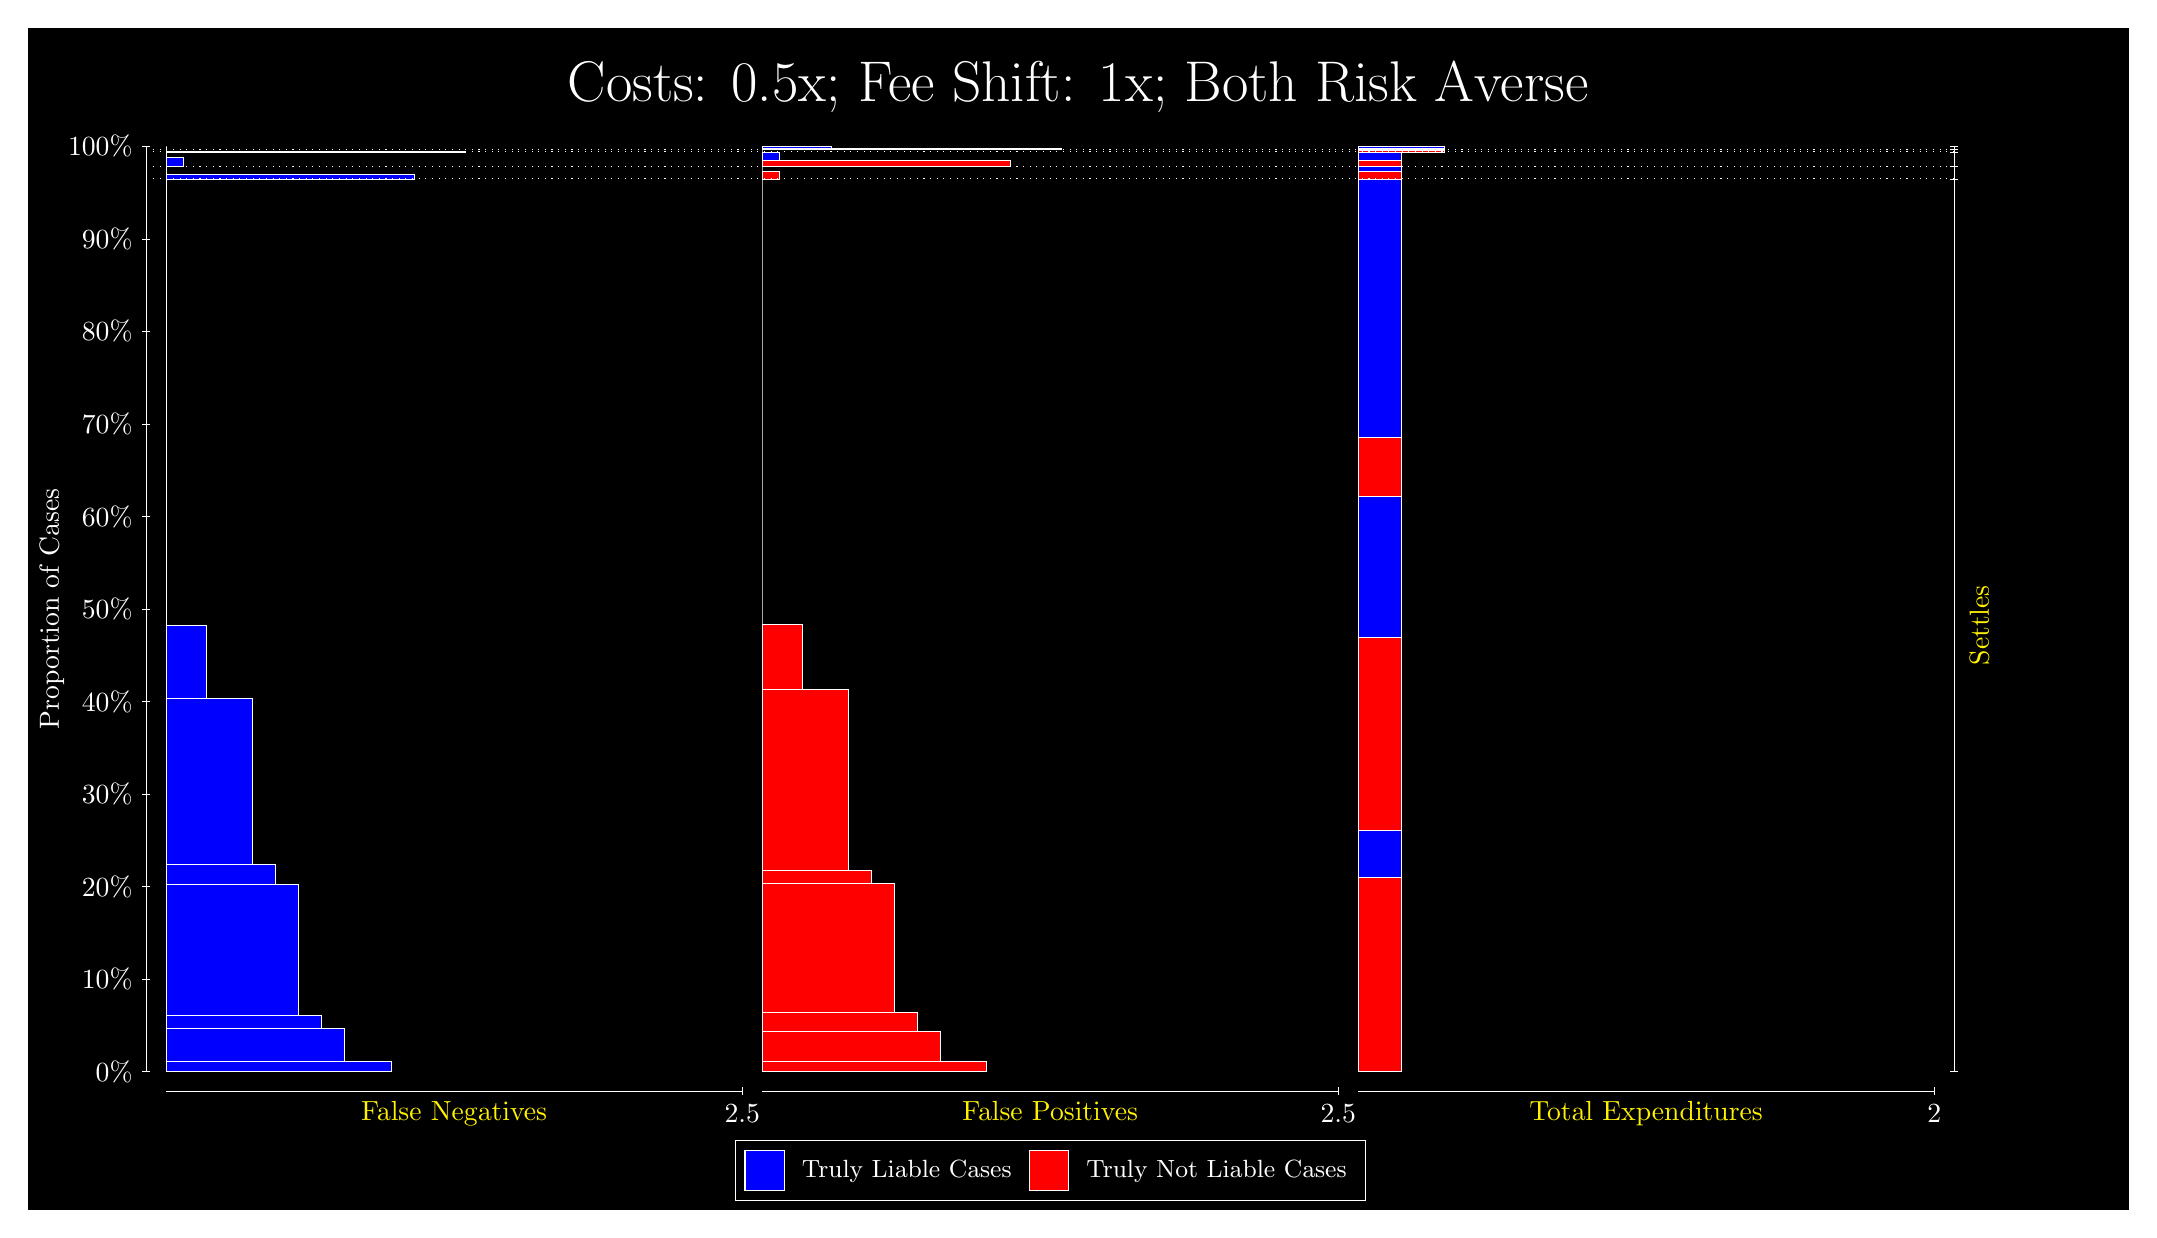
\begin{tikzpicture}
\draw[fill=black] (0,0) rectangle (26.667,15);
\draw[text=white] (0,13.5) rectangle (26.667,15) node[midway] {\huge Costs: 0.5x; Fee Shift: 1x; Both Risk Averse};
\draw[white, very thin] (1.5,1.75) -- (1.5,13.5);
\node[rotate=90, text=white, anchor=center] at (0.3, 7.625) {Proportion of Cases};
\draw[white, very thin] (1.45,1.75) -- (1.55,1.75);
\node[text=white, anchor=east] at (1.45, 1.75) {0\%};
\draw[white, very thin] (1.45,2.925) -- (1.55,2.925);
\node[text=white, anchor=east] at (1.45, 2.925) {10\%};
\draw[white, very thin] (1.45,4.1) -- (1.55,4.1);
\node[text=white, anchor=east] at (1.45, 4.1) {20\%};
\draw[white, very thin] (1.45,5.275) -- (1.55,5.275);
\node[text=white, anchor=east] at (1.45, 5.275) {30\%};
\draw[white, very thin] (1.45,6.45) -- (1.55,6.45);
\node[text=white, anchor=east] at (1.45, 6.45) {40\%};
\draw[white, very thin] (1.45,7.625) -- (1.55,7.625);
\node[text=white, anchor=east] at (1.45, 7.625) {50\%};
\draw[white, very thin] (1.45,8.8) -- (1.55,8.8);
\node[text=white, anchor=east] at (1.45, 8.8) {60\%};
\draw[white, very thin] (1.45,9.975) -- (1.55,9.975);
\node[text=white, anchor=east] at (1.45, 9.975) {70\%};
\draw[white, very thin] (1.45,11.15) -- (1.55,11.15);
\node[text=white, anchor=east] at (1.45, 11.15) {80\%};
\draw[white, very thin] (1.45,12.325) -- (1.55,12.325);
\node[text=white, anchor=east] at (1.45, 12.325) {90\%};
\draw[white, very thin] (1.45,13.5) -- (1.55,13.5);
\node[text=white, anchor=east] at (1.45, 13.5) {100\%};

\draw[white, very thin] (24.457,1.75) -- (24.457,13.5);
\draw[white, very thin] (24.407,1.75) -- (24.507,1.75);
\node[anchor=west] at (24.407, 1.75) {};
\draw[white, very thin] (24.407,13.086) -- (24.507,13.086);
\node[anchor=west] at (24.407, 13.086) {};
\draw[white, very thin] (24.407,13.248) -- (24.507,13.248);
\node[anchor=west] at (24.407, 13.248) {};
\draw[white, very thin] (24.407,13.43) -- (24.507,13.43);
\node[anchor=west] at (24.407, 13.43) {};
\draw[white, very thin] (24.407,13.465) -- (24.507,13.465);
\node[anchor=west] at (24.407, 13.465) {};
\draw[white, very thin] (24.407,13.5) -- (24.507,13.5);
\node[anchor=west] at (24.407, 13.5) {};

\draw[white, very thin, fill=blue] (1.75,1.75) rectangle (4.6044,1.8759);
\draw[white, very thin, fill=blue] (1.75,1.8759) rectangle (4.0188,2.3026);
\draw[white, very thin, fill=blue] (1.75,2.3026) rectangle (3.7261,2.4689);
\draw[white, very thin, fill=blue] (1.75,2.4689) rectangle (3.4333,4.1339);
\draw[white, very thin, fill=blue] (1.75,4.1339) rectangle (3.1406,4.3833);
\draw[white, very thin, fill=blue] (1.75,4.3833) rectangle (2.8478,6.496);
\draw[white, very thin, fill=blue] (1.75,6.496) rectangle (2.2623,7.4115);
\draw[white, very thin, fill=red] (1.75,7.4115) rectangle (1.75,13.086);
\draw[white, very thin, fill=blue] (1.75,13.086) rectangle (4.8971,13.151);
\draw[white, very thin, fill=red] (1.75,13.151) rectangle (1.75,13.248);
\draw[white, very thin, fill=blue] (1.75,13.248) rectangle (1.9696,13.362);
\draw[white, very thin, fill=red] (1.75,13.362) rectangle (1.75,13.43);
\draw[white, very thin, fill=blue] (1.75,13.43) rectangle (5.5558,13.442);
\draw[white, very thin, fill=red] (1.75,13.442) rectangle (1.75,13.465);
\draw[white, very thin, fill=red] (1.75,13.465) rectangle (1.75,13.477);
\draw[white, very thin, fill=blue] (1.75,13.477) rectangle (1.75,13.5);
\draw[white, very thin, fill=red] (9.3189,1.75) rectangle (12.173,1.8841);
\draw[white, very thin, fill=red] (9.3189,1.8841) rectangle (11.588,2.2571);
\draw[white, very thin, fill=red] (9.3189,2.2571) rectangle (11.295,2.5066);
\draw[white, very thin, fill=red] (9.3189,2.5066) rectangle (11.002,4.1347);
\draw[white, very thin, fill=red] (9.3189,4.1347) rectangle (10.709,4.301);
\draw[white, very thin, fill=red] (9.3189,4.301) rectangle (10.417,6.6039);
\draw[white, very thin, fill=red] (9.3189,6.6039) rectangle (9.8312,7.4244);
\draw[white, very thin, fill=blue] (9.3189,7.4244) rectangle (9.3189,13.086);
\draw[white, very thin, fill=red] (9.3189,13.086) rectangle (9.5384,13.183);
\draw[white, very thin, fill=blue] (9.3189,13.183) rectangle (9.3189,13.248);
\draw[white, very thin, fill=red] (9.3189,13.248) rectangle (12.466,13.317);
\draw[white, very thin, fill=blue] (9.3189,13.317) rectangle (9.5384,13.43);
\draw[white, very thin, fill=red] (9.3189,13.43) rectangle (9.3189,13.454);
\draw[white, very thin, fill=blue] (9.3189,13.454) rectangle (9.3189,13.465);
\draw[white, very thin, fill=red] (9.3189,13.465) rectangle (13.125,13.477);
\draw[white, very thin, fill=blue] (9.3189,13.477) rectangle (10.197,13.5);
\draw[white, very thin, fill=red] (16.888,1.75) rectangle (17.437,4.2192);
\draw[white, very thin, fill=blue] (16.888,4.2192) rectangle (17.437,4.8121);
\draw[white, very thin, fill=red] (16.888,4.8121) rectangle (17.437,7.2608);
\draw[white, very thin, fill=blue] (16.888,7.2608) rectangle (17.437,9.0517);
\draw[white, very thin, fill=red] (16.888,9.0517) rectangle (17.437,9.8082);
\draw[white, very thin, fill=blue] (16.888,9.8082) rectangle (17.437,13.086);
\draw[white, very thin, fill=red] (16.888,13.086) rectangle (17.437,13.183);
\draw[white, very thin, fill=blue] (16.888,13.183) rectangle (17.437,13.248);
\draw[white, very thin, fill=red] (16.888,13.248) rectangle (17.437,13.317);
\draw[white, very thin, fill=blue] (16.888,13.317) rectangle (17.437,13.43);
\draw[white, very thin, fill=red] (16.888,13.43) rectangle (17.986,13.454);
\draw[white, very thin, fill=blue] (16.888,13.454) rectangle (17.986,13.465);
\draw[white, very thin, fill=red] (16.888,13.465) rectangle (17.986,13.477);
\draw[white, very thin, fill=blue] (16.888,13.477) rectangle (17.986,13.5);
\draw[white, dotted] (1.5,13.086) -- (24.457,13.086);
\draw[white, dotted] (1.5,13.248) -- (24.457,13.248);
\draw[white, dotted] (1.5,13.43) -- (24.457,13.43);
\draw[white, dotted] (1.5,13.465) -- (24.457,13.465);
\draw[white, very thin] (1.75,1.5) -- (9.0689,1.5);
\node[text=yellow, anchor=north] at (5.4094, 1.5) {False Negatives};
\draw[white, very thin] (9.0689,1.45) -- (9.0689,1.55);
\node[text=white, anchor=north] at (9.0689, 1.45) {2.5};

\draw[white, very thin] (9.3189,1.5) -- (16.638,1.5);
\node[text=yellow, anchor=north] at (12.978, 1.5) {False Positives};
\draw[white, very thin] (16.638,1.45) -- (16.638,1.55);
\node[text=white, anchor=north] at (16.638, 1.45) {2.5};

\draw[white, very thin] (16.888,1.5) -- (24.207,1.5);
\node[text=yellow, anchor=north] at (20.547, 1.5) {Total Expenditures};
\draw[white, very thin] (24.207,1.45) -- (24.207,1.55);
\node[text=white, anchor=north] at (24.207, 1.45) {2};

\node[text=yellow, centered, rotate=90] at (24.777, 7.4179) {Settles};





\draw (12.978300999999998,1.5) node[draw=none] (baseCoordinate) {};
\begin{scope}[align=center]
        \matrix[scale=0.5, draw=white, below=0.5cm of baseCoordinate, nodes={draw}, column sep=0.1cm]{
            \node[rectangle, draw, minimum width=0.5cm, minimum height=0.5cm, fill=blue] {}; &
            \node[draw=none, font=\small, text=white] (B) {Truly Liable Cases}; &
            \node[rectangle, draw, minimum width=0.5cm, minimum height=0.5cm, fill=red] {}; &
            \node[draw=none, font=\small, text=white] (B) {Truly Not Liable Cases}; \\
            };
\end{scope}

\end{tikzpicture}
\end{document}